\section{Experimental Evaluation}
\label{sec:experiments}
In this section we present both qualitative and quantitative  performance evaluations of visual MPC on various manipulation tasks, comparing different prediction models and cost functions.



\noindent \textbf{Qualitative Evaluation}
In figure \todo{add figure} we show a series of qualitative experiments showing that visual MPC trained fully self-supervised is capable of solving a wide range of complex tasks:
\todo{adapt these points}
\begin{enumerate}
	\item Multiple-object relocation tasks through pushing
	\item Combined obstacle avoidance and object relocation tasks in the presence of occlusion
	\item Object relocation through combined pushing and grasping
	\item Object relocation task with external perturbations of the object position
	\item Relative object rearrangment tasks, including multiple object rearrangement
	\item Handling of deformable objects, such as towel folding and cloth folding
\end{enumerate}
Videos for the qualitative examples are provided on the following webpage: \url{https://sites.google.com/view/visualforesight/}

\noindent \textbf{Quantitative Evaluation} We define a set of benchmark tasks where the robot is required to move objects in its environment from a starting state to a goal configuration. For measuring success, we use a distance based evaluation where a human annotates the positions of the objects after pushing allowing us to compute the remaining distance to the goal.
%\begin{enumerate}
%	\item [\ref{subsec:sna_experiments}] How important is the model's ability to handle occlusion? How do temporal skip-connections introduced in the SNA-model affect performance compared to the DNA model without skip-connections?
%	\item [\ref{susbsec:reg_cost_exp}] How important is the system's ability to update the belief of \emph{where} the object is? How is performance affected by using a registration-based cost function, and how does closed-loop visual MPC compare to closed-loop visual MPC and visual MPC with off-the-shelf tracking?
%	\item [\ref{subsec:eval_classifier}] How does visual MPC with a classifier-based cost function compare to visual MPC with pixel MSE-based cost function on relative object rearrangement tasks?
%	\item [\ref{subsec:multi_task_bench}] How does visual MPC compare to a hand-engineered controller that relies on a calibrated camera on a large set of diverse tasks?
%\end{enumerate}

%%SL.10.16: Put all these boring details into some subsection titled something like Experimental Setup. However, a lot of this is actually supposed to be covered in Section 7 above -- it's a bit weird to have a bunch more experimental setup now in this section. Maybe try to collect it all in one place?



\subsection{Comparing different Video-Prediction Architectures}
\label{subsec:sna_experiments}
Here we answer the question: Does  visual-MPC using the occlusion-aware SNA video prediction model that includes temporal skip connections outperform visual MPC with the dynamic neural advection model (DNA)\cite{foresight} \emph{without} temporal skip-connections?
We evaluate on multi-objective tasks where one object must be pushed without disturbing another.

	%%SL.10.16: This sounds really disappointing. Presumably we do lots of other cool stuff too? What about classifier, towels, rearrangement and placing tasks?
	
	%%SL.10.16: do we use the same test procedure in other subsections too? If so, let's have a separate subsection to describe the experiment, and then separate subsections for results, otherwise there will be a lot of duplication. Don't just staple the experiment sections from different papers together...
	%\todo{\autoref{fig:long_distance_task} shows an example task for the pushing benchmark.}
	%%SL.10.16: I think these "bare bones" pictures with no distractors are really boring. Can we mostly show interesting tasks with lots of distractors, and contain the simple pushing tasks in one subsection? If we have lots of pictures of the simple tasks, people will conclude that the method only works with one object in the scene.
	%We collected 20 trajectories with 3 novel objects and 1 training object. \autoref{table:res_dna_sna} shows the results for the pushing benchmark. The column \textit{distance} refers to the mean distance between the goal pixel and the designated pixel at the final time-step. The column \textit{improvement} indicates how much the designated pixel of the objects was moved closer to their goal (or further away for negative values) compared to the starting location. The true locations of the designated pixels after pushing were annotated by a human labeler.
	
	%The results in \autoref{table:res_dna_sna} show that our proposed planning cost in \autoref{eq:cost}
	%%SL.10.16: wait, what? I thought this section was evaluating models, not costs? Can we separate these out, first evaluate models, then costs, to reflect the organization in the paper?
	%substantially outperforms the planning cost used in prior work~\cite{foresight}. The performance of the SNA model in these experiments is comparable to the DNA model~\cite{foresight} when both use the expected-distance planning cost, since this task does not involve any occlusions.
	%%SL.10.16: Hmm... OK, perhaps if we're going to evaluate costs and models simultaneously like this, we need to organize the sections more clearly. Maybe it would really help in that case to separate out experiment setup (how the methods care compared) from the results (how they stack up). And for each section, ask yourself: what is the question these experiments are trying to answer? It should be obvious from the writing. Right now, I feel like the experiments section looks too much like experiments sections from different papers stapled together. They need to more integrated and focused on achieving the paper's aims: state the research questions, and explain how each experiment subsection answers one or more of those questions



\begin{table}
\centering
{\footnotesize
\begin{tabular}{lcc}
	\toprule
         &  \thead{moved imp. \\ $\pm$ std err. of mean} &   \thead{stationary imp. \\ $\pm$ std err. of mean}  \\
         \midrule
  DNA \cite{foresight} & 0.83 $\pm$0.25 &  -1.1 $\pm$ 0.2\\ 
  SNA & \textbf{10.6 $\pm$ 0.82} & \textbf{-1.5 $\pm$ 0.2} \\
  \bottomrule
\end{tabular}
}
\caption{Results for multi-objective pushing on 8 object/goal configurations with 2 seen and 2 novel objects. Values indicate improvement in distance from starting position, higher is better. Units are pixels in the 64x64 images.} 
\label{table:mult_obj}
\end{table}

To examine whether our skip-connection model (SNA) helps with handling occlusions, we devised a task that requires the robot to push one object, while keeping another object stationary. When the stationary object is in the way, the robot must move the target object around it. This is illustrated in  \autoref{fig:goingaroundocclusion} on the left in the appendix. While doing this, the gripper may occlude the stationary object, and the task can only be performed successfully if the model can make accurate predictions through this occlusion. These tasks are specified by picking one pixel on the target object, and one on the obstacle. The obstacle is commanded to remain stationary, by choosing the target position to be at the same location as the initial position. For the target object the destination is chosen on the other side of the obstacle.

We used four different object arrangements, with two training objects and two objects that were not seen during training. We found that, in most of the cases, the SNA model was able to find a valid trajectory, while the DNA model, that is not able to handle occlusion, and was mostly unable to find a solution. The results of our quantitative comparisons are shown in \autoref{table:mult_obj}, indicating that temporal skip-connections indeed help with handling occlusion in combined pushing and objstacle avoidance tasks. See a more detailed explanation of the experiment in the appendix.


%%SL.10.16: It would help if the experimental conclusion at the end of this section is an answer to  question posed earlier in the experiments. I also think it makes too big of a deal out of the SNA thing -- this is not the SNA paper, we don't need to push on this so hard!

\subsection{Evaluating Registration-based Cost Function}
\label{susbsec:reg_cost_exp}
%%SL.10.16: This is very misleading, all of the experiments are closed-loop!

\begin{table}
	{\footnotesize
		\begin{center}
			\begin{tabular}{lcc}
				\toprule
				%				 & \multicolumn{2}{c}{fraction of successful runs} \\
				& Short & Long \\
				\midrule
				Visual MPC $+$ predictor propagation  & 83\% & 20\% \\
				Visual MPC $+$ OpenCV tracking  & 83\%  & 45\% \\
				Visual MPC $+$ registration network & 83\% & \textbf{66\%}  \\
				\bottomrule
			\end{tabular}
		\end{center}
	}
	\caption{\small Success rate for long-distance pushing benchmark with 20 different object/goal configurations and short-distance benchmark with 15 object/goal configurations. Success is defined as bringing the object closer than 15 pixels to the goal, which corresponds to around $7.5cm$.}
	\label{table:res_long_short}
\end{table}

\todo{put in example explaining push with perturbation, why is this worth studying?}

In this section we are concerned with: \emph{How important} quantitatively is it to update the model's belief of where the target objects currently are? How much does this matter for short versus horizon tasks?
In this experiment, we disable the gripper control, which requires the robot to push objects to the target. We compare two variants of updating the positions of the designated pixel when using a pixel-distance based cost function. The first one is a cost function that uses a registration-based method, trained in a fully-self-supervised fashion an the second one is with a cost function that uses off-the shelf tracking from OpenCV \cite{babenko2009visual}. Additionally we compare to visual-MPC that uses the video-prediction model's own predictions as the current positions of the designated pixel, rather than tracking the object.

%SL.10.16: Before talking about videos, explain what this experiment section is actually studying! What is the question? What are you evaluating? Why?

%%SL.10.16: again, not entirely clear what question this is trying to answer

\begin{figure*}
    \centering    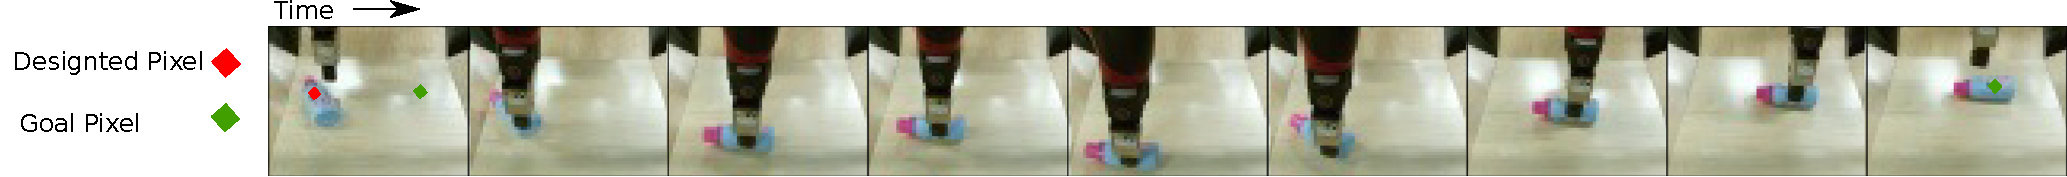
\includegraphics[width=1.0\textwidth]{images_rfr/push_correction.pdf}
    \caption{\small{Applying our method to a pushing task. In the first 3 time instants the object behaves unexpectedly, moving down. The tracking then allows the robot to retry, allowing it to eventually bring the object to the goal.}}
    \label{fig:push_retry}
\end{figure*}

%\begin{figure}
%	\centering
%	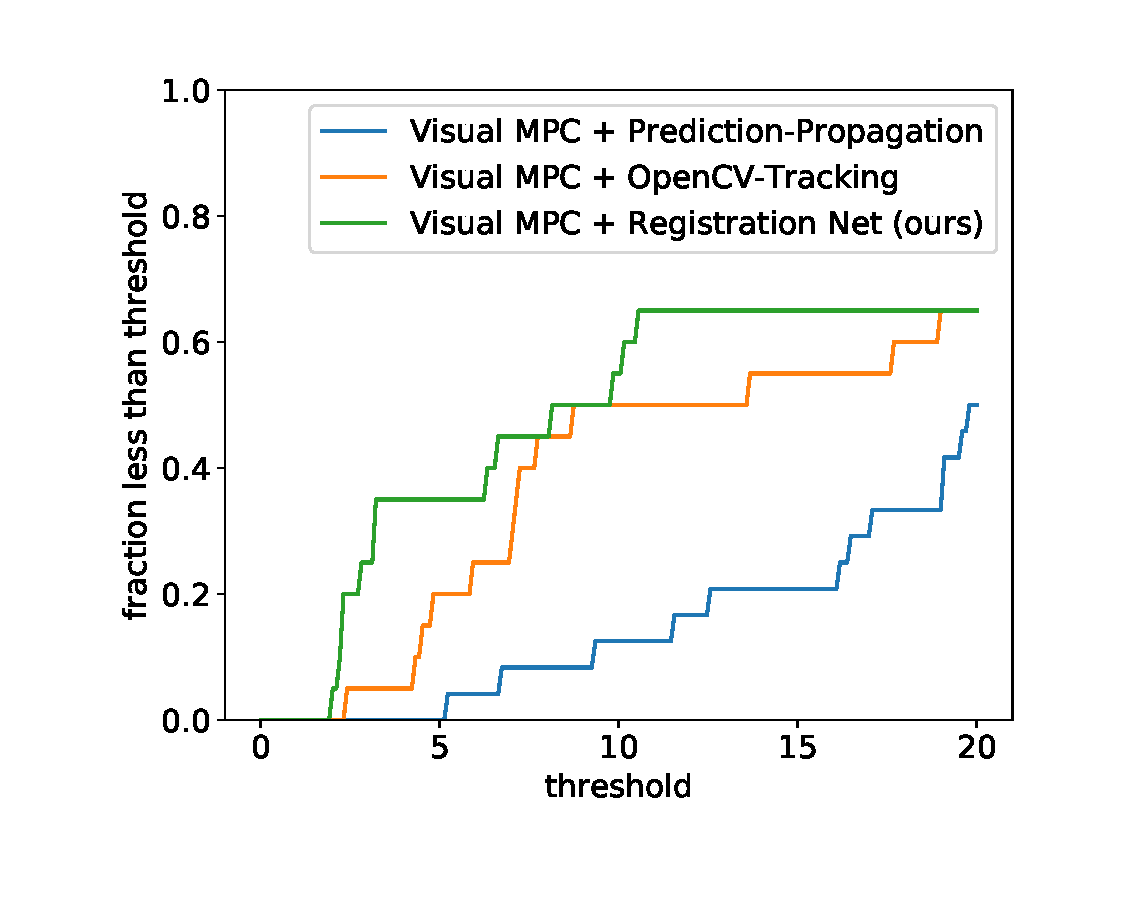
\includegraphics[width=0.8\columnwidth]{images_rfr/pushlong_bench_same_range.pdf}
%	\caption{\small{Results for long pushing tasks with 20 objects not seen during training, showing fraction of runs where final distance is lower than threshold. Our method shows a clear gains over OpenCV tracking and predictor propagation.}}
%	\label{fig:push_bench_long}
%\end{figure}

We evaluate our method on 20 long-distance and 15 short-distance pushing tasks. For long-distance tasks the distance between the object and its goal-position is $30cm$ while for short-distance tasks it is $15cm$. Table \ref{table:res_long_short} lists quantitative comparisons showing that on the long-distance benchmark visual-MPC using the registration-based cost not only outperforms prior work \cite{sna}, but also outperforms the hand-designed, supervised object tracker \cite{babenko2009visual}. By contrast for the short distance benchmark, all methods perform comparably. Thus theses results demonstrate the importance of closed loop control for \emph{long-horizon tasks}, while for short-horizon tasks object tracking appears to be irrelevant. Furthermore using the learned registration, the robot is more frequently able to successfully recover after erroneous predictions or occlusions, an example is shown in \autoref{fig:push_retry}.

\begin{figure*}
	\centering
	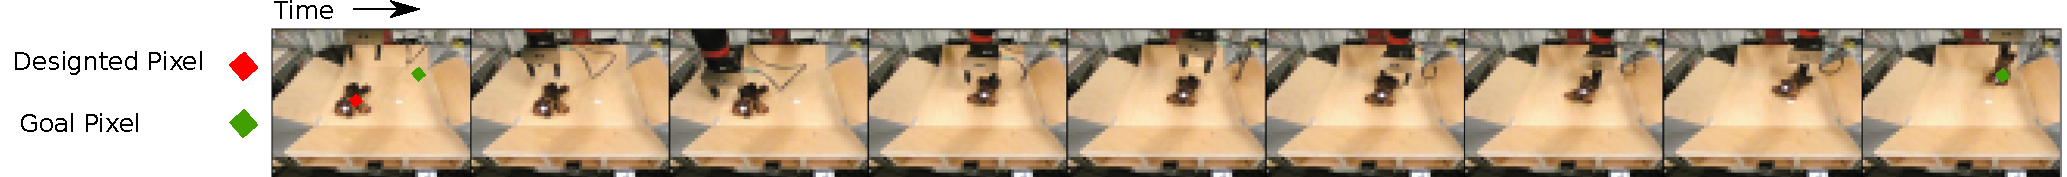
\includegraphics[width=1.0\textwidth]{images_rfr/pick_place_plush.pdf}
	\caption{\small{Retrying behavior of our method combining prehensile and non-prehensile manipulation. In the first 4 time instants shown the robot pushes the object. It then loses the object, and decides to grasp it pulling it all the way to the goal. Retrying is enabled by applying the learned registration to both camera views (here we only show the front view).}}
	\label{fig:push_grasp}
	
\end{figure*}

\subsection{Evaluating Classifier-based Cost Function}
\label{subsec:eval_classifier}

Here we study the question: How does the success rate of visual MPC using the proposed classifier-based cost function in a relative object arrangement task compare to a baseline based on pixel-distance and DSAE?

%We evaluate our learned classifier on the predictions made by the video prediction model \todo{unclear, how exactly do you evaluate the classifier?} and derive the cost used for planning from the predicted probability of success. 

To collect data for meta-training the classifier, we randomly select a pair of objects from our set of training objects, and position them into many different relative positions, recording the image for each configuration. One task corresponds to a particular relative positioning of two objects, e.g. the first object to the left of the second, and we construct positive and negative examples for this task by labeling the aforementioned images. We randomly position the arm in each image, as it is not a determiner of task success. A good objective should ignore the position of the arm. We also include randomly-positioned distractor objects in about a third of the collected images.

We evaluate all approaches in three different experimental settings. In the first setting, the goal is to arrange two objects into a specified relative arrangement. The second setting is the same, but with distractor objects present. In the final, most challenging setting, the goal is to achieve two tasks in sequence. We provide positive examples for both tasks, infer the classifier for both task, perform MPC for the first task until completion, followed by MPC for the second task. To evaluate the ability to generalize to new goals and settings, we use novel, held-out objects for all of the task and distractor objects in our evaluation. 

We qualitatively visualize the benchmark tasks in Figure~\ref{fig:cls_results} in the appendix.

On the left, we show a subset of the five images provided to illustrate the task(s), and on the left, we show the motions performed by the robot. We see that the robot is able to execute motions which lead to a correct relative positioning of the objects. \todo{refrence exmaple trajectories}

We quantitatively evaluate each method across 20 tasks, including $10$ unique object pairs. The results, shown in Figure~\ref{fig:cls_charts}, indicate that prior methods for learning distance metrics
%%SL.10.16: you mean the method *in this paper*?
struggle to infer the goal of the task, while our approach leads to substantially more successful behavior on average. 
\todo{explain how exactly you measure success} 
%%SL.10.16: what is the conclusion from all this? how do the different methods of specifying costs stack up?

%%SL.10.16: where are qualitative results and discussion of cloth?


\begin{figure}
    \centering
    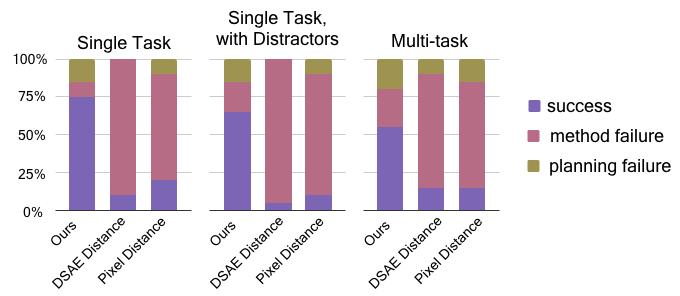
\includegraphics[width=0.48\textwidth]{images_cls/cls_charts.jpeg}
    \caption{\small Quantitative performance of visual planning for object rearrangement tasks across different goal specification methods: our meta-learned classifier, DSAE~\cite{finn_nips} \todo{what is DSAE?}, and pixel error. Where possible, we include break down the cause of failures into errors caused by inaccurate prediction or planning and those caused by an inaccurate goal classifier.}
    \label{fig:cls_charts}
    \vspace{-0.3cm}
\end{figure}


\subsection{Multi-Task Benchmark}
\label{subsec:multi_task_bench}
In this benchmark we  assess the capability of visual MPC to handle a \emph{wide range of tasks} without problem-specific parameter tuning. We seek to answer the question: How does visual MPC compare to a hand-engineered baseline on a large number of diverse tasks? 
%The following types of tasks were included in the benchmark.
%\begin{itemize}
%\item picking up an object and placing into container
%\item folding cloths, i.e. shirts and shorts
%\item picking up and object and bringing it into a desired 3D configuration
%\item pushing an object to a desired location
%\item wrap a towel around an object
%\item rotate a piece of cloth around the vertical axis
%\end{itemize}
Alltogether 16 tasks were selected, figure \todo{ref figure with examples} shows the execution of visual MPC on these tasks. 

\noindent \textbf{Hand-crafted Baseline} A simple trajectory generator was engineered to perform a grasp at the location of the initial designated pixel, lift the arm and bring it to the position of the goal-pixel. A camera calibration was performed to carry out the necessary conversions between image-space and robot work-space coordinates. For simplicity, the baseline controller executes open-loop. Therefore to allow for a fair comparison visual-MPC is also executed open-loop, i.e. no registration or tracking is used.

The results of the benchmark, shown in table \ref{table:cloth_folding}, indicate that visual MPC clearly outperforms the baseline. 
Visual MPC succeeded for most of the benchmark tasks. While the baseline succeeded for some of the cloth folding tasks, it failed for almost all of the object relocation tasks. We attribute this to the fact that it does not have a model, therefore it is lacking the capability of positioning the endeffector in a location that is appropriate for grasping or pushing. 
\todo{put in refs to example trajecotries!}

\label{subsec:cloth_folding_data}
\begin{table}
\centering
{\footnotesize
\begin{tabular}{lcc}
	\toprule
         &  \thead{\% of Trials with \\ Final Pixel Distance $< 15$}   \\
         \midrule
  Visual MPC & \textbf{75\%} \\ 
  Calibrated Camera Baseline & 18.75 \% \\
  \bottomrule
\end{tabular}
}
\caption{Results for a combined benchmark of 10 hard object pushing and grasping tasks, along with 6 cloth folding tasks. Values indicate the percentage of trials which ended with the object closer than a threshold distance (measured in pixels) to the designated goal. Higher is better.} 
\label{table:cloth_folding}
\end{table}